
\subsection{Determining block size}


\begin{figure}[t]
    \centering
    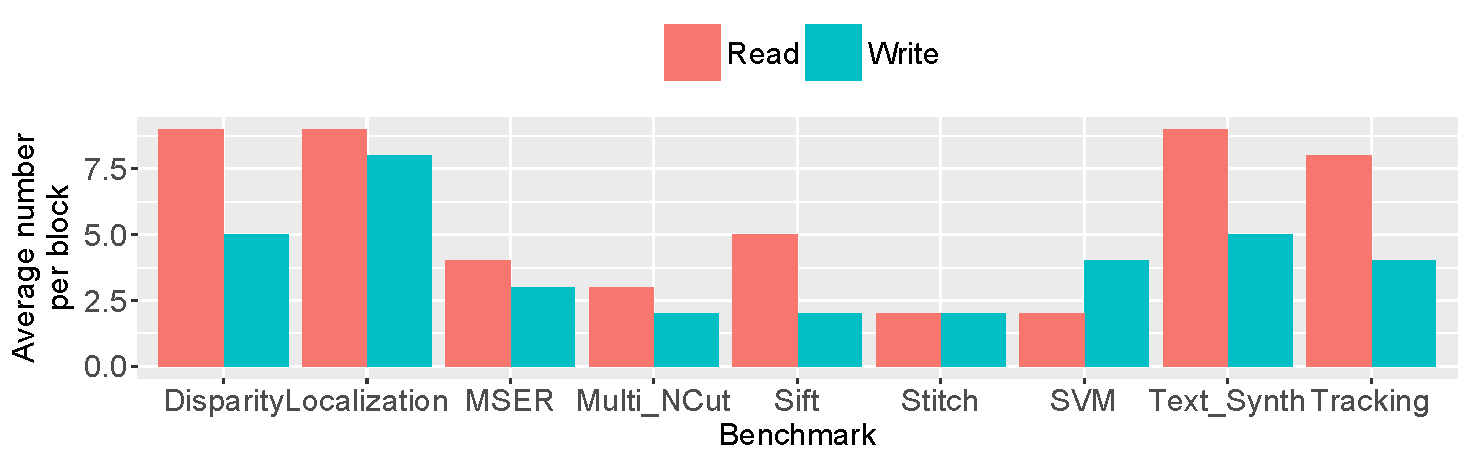
\includegraphics[width=1\textwidth]{chapter3/graphics/averageRegRead.pdf}

    \caption{Average number of register reads and writes per EDGE block.}
    \label{fig:edge_reg_read}
	\vspace{1em}
\end{figure}
One of the defining factors of the block based D-VTAGE predictor is that a single prediction fetches a fix set of values rather than requiring one request per instruction.
Due to the fact that the block size is fixed, determining the correct size is important.
Having a large block size means that the D-VTAGE predictor can predict all values in a block, however this comes at the sacrifice of having less blocks in memory.
On the other hand, small block size allows to have multiple blocks stored at a time but may require values of an EDGE block to be found in multiple D-VTAGE blocks.
This would increase the number of requests to the value predictor, which may become a bottleneck.

In this chapter, the value predictor is focused on register reads rather than load-store operations.
This is due to the fact that, unless the load-store dependence predictor detects a data dependency between two blocks, memory operations operate in parallel.
Focussing only on register reads will reduce the the block size requirements as reads tend to be a minor component of an EDGE block.
To determine the block size, all the EDGE blocks of the SD-VBS benchmarks are anaylsed to find out the what the average register read and write count is per block.
The writes are also tracked as it provides information on the potential amount of register dependencies found in each of the applications.

Figure~\ref{fig:edge_reg_read} shows the average number of register read and writes for each of the benchmarks.
On average, there are 5 register reads and 3 register writes per block.
Whilst \bm{Disparity} \bm{Localization}, \bm{Texture\_Synthesis} and \bm{Tracking} have higher register read counts than the average, most of them only have 5 writes per block.
This potentially means that having a D-VTAGE block size of 5 would capture all dependencies.
However this would require either compiler analysis to mark register reads that potentially need value prediction, or have hardware to detect patterns of data-dependencies.
This work is left for future endeavours.
To summarise, iff the block size is too small, this means that some reads cannot be predicted, whilst if the blocks are too large this reduces the number of entries in the D-VTAGE tables, limiting the coverage.

\subsection{Block variation analysis}

\begin{figure}[t]
    \centering
    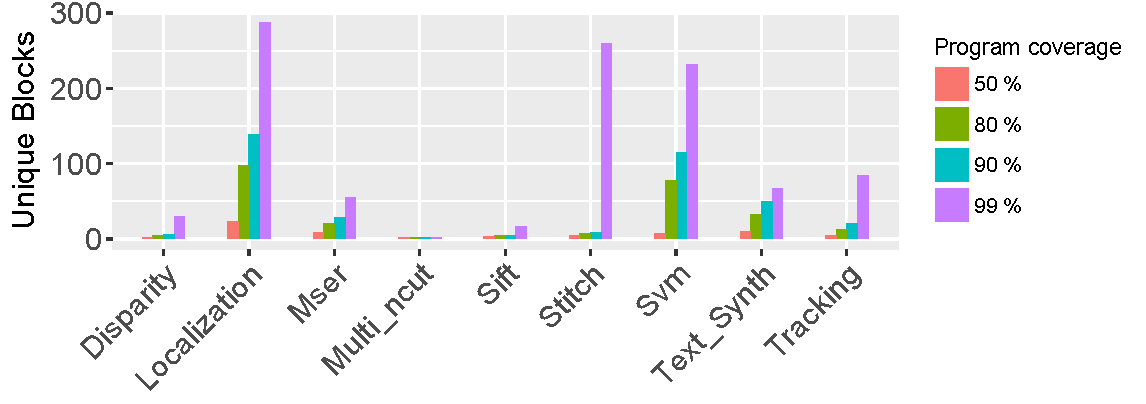
\includegraphics[width=1\textwidth]{chapter3/graphics/unique_blocks.pdf}

    \caption{Number of unique blocks comprising different percentages of the total execution (in blocks) of each of the benchmarks.}
    \label{fig:totblock}
	\vspace{1em}
\end{figure}

One method of understanding how the block based D-VTAGE predictor will perform is to study the number of unique blocks found in each of the benchmarks.
Benchmarks that feature a smaller number of unique blocks can potentially benefit more from value prediction as the predictor cannot hold many blocks at a time.
Reporting all unique blocks executed is not a proper evaluation of the variety of blocks found in the benchmark, as some will most certainly be executed more times than other.
To account for this, blocks are sorted by number of occurences, and then added to the unique block count as long as their occurences are under a variable percentage of the total number of blocks executed.

Figure~\ref{fig:totblock} shows the number of unique blocks found in each benchmark that represent 50,80,90 and 99\% of the total number of executed blocks.
As can be seen, applications \bm{Disparity}, \bm{Multi\_NCut} and \bm{Sift} \bm{Stitch} and \bm{Tracking} execute less than 50 unique blocks during 90\% of its total execution.
This is promising as it means that there is a high chance that the predictor requires less entries to capture all possible blocks in the application.
On the other hand, \bm{Localization}, and \bm{SVM} execute over 100 blocks throughout 90\% of their execution, twice as many as the previously mentioned benchmarks.
For these applications, it migth be harder to predict values as new blocks may overwrite entries in the predictor.

\subsection{Setup}
This section demonstrates how the block based D-VTAGE value predictor improves the performance of core composition, with the round-robin fetch scheme (RRF).
Serial fetch is not explored as the previous section showed that when considering value prediction, RRF always provides the best results.

The objective of this section is to demonstrate that a state of the art value predictor can be used to improve the performance of large core compositions, and to show the difference between a real predictor and the perfect predictor.
The D-VTAGE size configuration can be found in Table~\ref{tab:vtage-conf}.
The total number of entries for the D-VTAGE predictor is taken from Perais et al's original paper which introduced the predictor~\cite{peraisBeBop2015}.
For the size of the stride, 64bit values were used throughout the experiments, to maximise the reach of the predictor.
However, different stride sizes are considered: the simulator tracks the size of the strides used in valid predictions to detect how small the strides can be made for each of the benchmarks.
The analysis of the stride size is discussed later on in this section.

For this section, two features of the predictor are modified: the number of entries per block and at what confidence a prediction is used.
Modifying the required confidence explores the trade-off beteween high coverage and low misprediction.
The original D-VTAGE paper uses Forward Probabilistic Counters (FPC)~\cite{riley2006fpc} to increment the confidence, and only used predictions once the counter was set to 7.
This section explores two counter scenarios: using a prediction when the confidence is set to 4 (without FPC), and using confidence when the counter is set to 7 (with FPC).
The FPC vector used in this Chapter is the same as the one in Perais et al.'s work $\{1,\frac{1}{16},\frac{1}{16},\frac{1}{16},\frac{1}{16},\frac{1}{16},\frac{1}{32},\frac{1}{32}\}$.
This confidence rate ensured that the predictor had an accuracy of over 99\%, but at the expense of a low coverage, 20\% on average~\cite{peraisBeBop2015}.
Table~\ref{tab:vtage-params} shows the possible values that can be taken for the two parameters.

\begin{table}[t]
  \small
  \centering
 \begin{tabular} {| l | l | l |}
 \hline
	\#Base Ent. & \#Tagged & \#Spec Window\\ \hline
	256 & $6\times256$ & 4 \\ \hline
	\end{tabular}
  \caption{D-VTAGE table configuration.}\label{tab:vtage-conf}
  \vspace{1em}
\end{table}


\begin{table}[t]
\small
\centering
\begin{tabular}{p{5.2cm} p{1.8cm}}
\toprule
\textbf{Parameter} & \textbf{Values} \\ \midrule
\# of entries per block & 8, 16\\
Confidence Value & 4 or 7 with FPC \\ \bottomrule
\end{tabular}
\caption{Configurable parameters for D-VTAGE}\label{tab:vtage-params}
\end{table}

\subsection{D-VTAGE Results}

\subsubsection{Performance}

\begin{figure}[t]
    \centering
    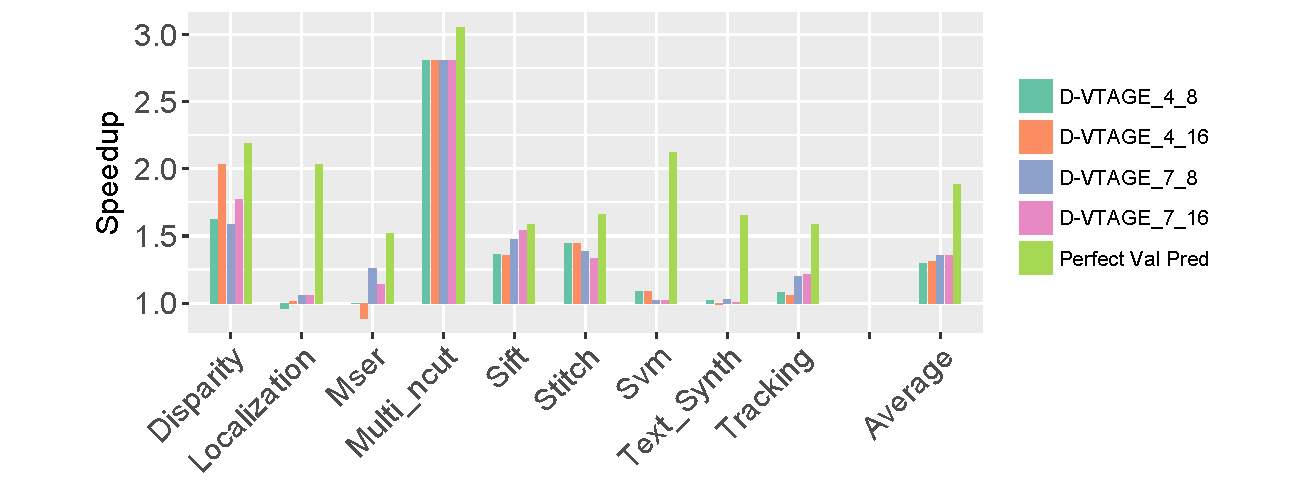
\includegraphics[width=1\textwidth]{chapter3/graphics/vtage_speed2.pdf}
    \caption{Comparing the performance of the standard fetching scheme to the new fetching scheme, with and without perfect value prediction. Higher is better.}
    \label{fig:vtage_perf}
	\vspace{1em}
\end{figure}

Figure~\ref{fig:vtage_perf} reports the speedup obtained with the different configurations of the D-VTAGE predictor.
The baseline is a 16 core composition that uses the serial fetching (SF) scheme without any value prediction and using perfect branch prediction.
The lack of value prediction and use of serial fetching mimicks the current implementation of core composition.
To better evaluate the predictor, each configuration is compared to the perfect predictor, which can predict every register value at any instance.

On average, using a D-VTAGE value predictor with a Round Robin fetching scheme results in a speedup of 1.32x.
When comparing the performance between the different configurations, the main observation is that using FPC and higher confidence trigger can impact performance.
This is most visibly seen for the benchmark \bm{Disparity} where using a higher confidence leads to a 1.75x speedup compared to 2.0x for a confidence counter of 4.
On the other hand, \bm{Localization} and \bm{MSER} performs worse with a lower confidence counter, and result in a slowdown.
Benchmarks \bm{Sift} and \bm{Tracking} perform better with a higher confidence, but the results of using a 4 bit counter never negatively impact performance.

When it comes to the size of a block, often the block with 16 entries does not lead to better performance than the one with 8 entries but stays on par with it.
The only noticeable difference is with \bm{MSER} where the smaller block performs better.

When comparing the performance of the different D-VTAGE configurations to the perfect value predictor, it shows that most benchmarks are not achieving their maximum potential.
This is most obvious with most benchmark as the perfect predictor results in an average speedup of 1.88x compared to 1.32x of D-VTAGE.
However, benchmarks \bm{Disparity} and \bm{Multi\_NCut} show how value prediction paired with RRF is a promising lead for improving the performance of core composition.

\subsubsection{Coverage and accuracy}
To better understand the performance of D-VTAGE, the predictor's coverage and misprediction rates are recorded.
Since EDGE is a block based architecture, it is important to study the coverage and accuracy on both a per-register read and per-block level.
This is due to the fact that a single read misprediction will lead to flushing the block and all younger blocks in the chain.
Thus whilst the misprediction rate for number of predicted instructions may be low, it can have a larger impact than on a traditional x86 machine.
Also a single accurate register prediction may not necessarily improve performance as that register may not have any dependencies with other live blocks.

\begin{figure}[t]
    \centering
    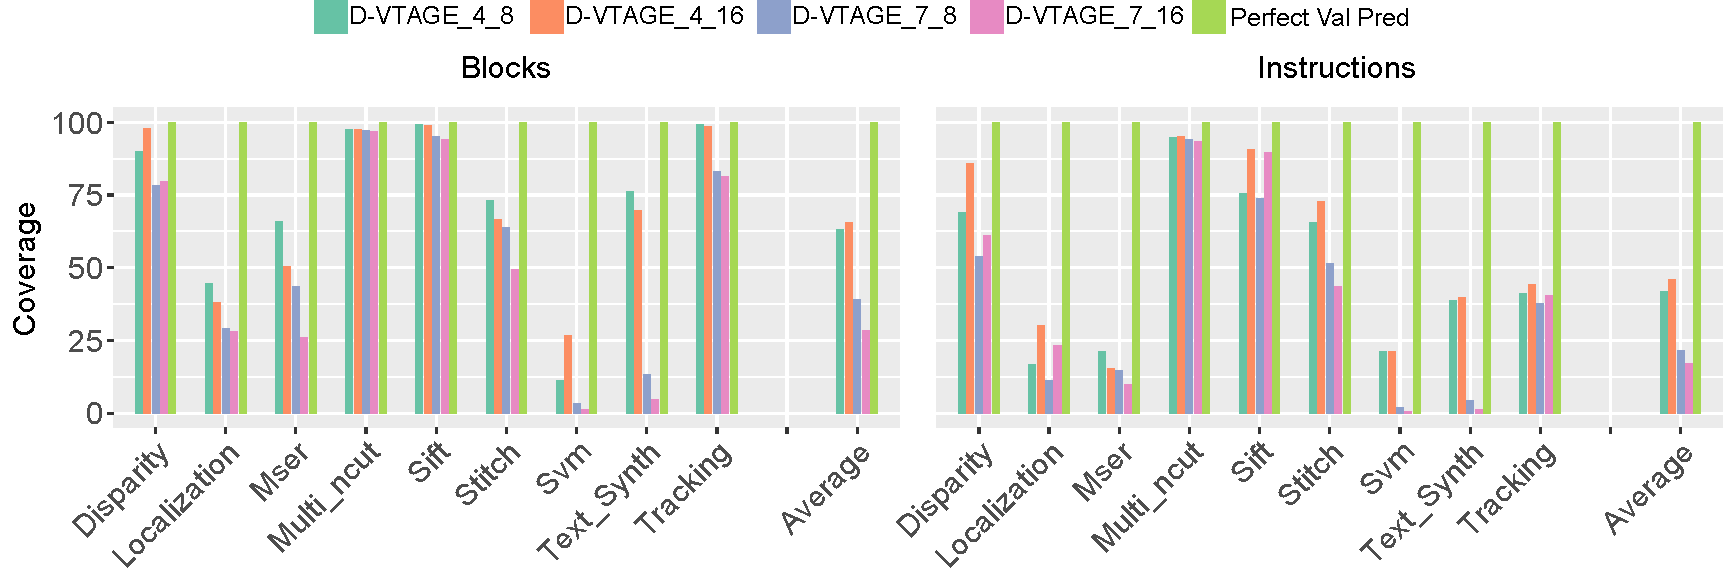
\includegraphics[width=1\textwidth]{chapter3/graphics/coverageFull.pdf}
    \caption{Prediction coverage at a block and instruction level. Higher is better}
    \label{fig:vtag_cov_block}
	\vspace{1em}
\end{figure}

Before looking at the accuracy of the predictors, it's important to study the coverage as it gives an overall view of how active the value predictor is during the execution of a program.
In this chapter, only blocks that are committed count towards the predicted blocks, as flushes caused by other issues such as LSQ violations may artificially inflate the coverage count.
Figure~\ref{fig:vtag_cov_block} shows the number of blocks which had at least one prediction, relative to the total number of committed blocks and the number of predicted register reads relative to the total executed register reads.
Both figures show similar patterns: the predictors with lower confidence counters have a higher coverage, 65\% compared to 31\% for the high confidence counter.
This is normal, as lower confidence causes predictions to be used with less training, and thus increases the number of predictions used during the execution of the program.

Whilst the block coverage is high, the coverage for registers shows that not all registers are being predicted (Figure~\ref{fig:vtag_cov_block}).
Once again, lower confidence equates to higher coverage, however this time it's 30\% for a confidence of 4 and under 25\% for a confidence of 7.
The register coverage for a confidence of 7 is in line with the coverage reported in Perais. et al's work ~\cite{peraisBeBop2015, peraisVTAGE2014} if not slightly higher.
The coverage may be slightly higher due to the fact that the values being predicted are often either loop increments or memory increments.

The register coverage helps explain why the high block coverage does not lead to better performance: whilst most blocks may have a valid prediction, some of the register reads cannot be predicted.
This may be due to data being carried over which is unpredictable.
For instance a loop which sums all values of an array into a single integer will pass that integer via a register.
This register will cause a data dependency between loop iterations and cannot be predicted unless the values in the array are highly predictable.

\bm{Localization}, \bm{MSER}, \bm{SVM} and \bm{Texture\_Synthesis} often have much lower coverage than the rest of the programs.
Recalling Figure~\ref{fig:totblock} which shows the number of unique blocks executed throughout the programs, these benchmarks had a higher count of unique blocks.
This explains why the coverage will be lower: there's a higher chance of encountering a new block than executing a known one.
As blocks require multiple executions to train the predictor (if the values in the register are indeed predictable), than the higher diversity of blocks makes it harder.
Thus, these benchmarks will naturally have a harder time to benefit from value prediction.


\begin{figure}[t]
    \centering
    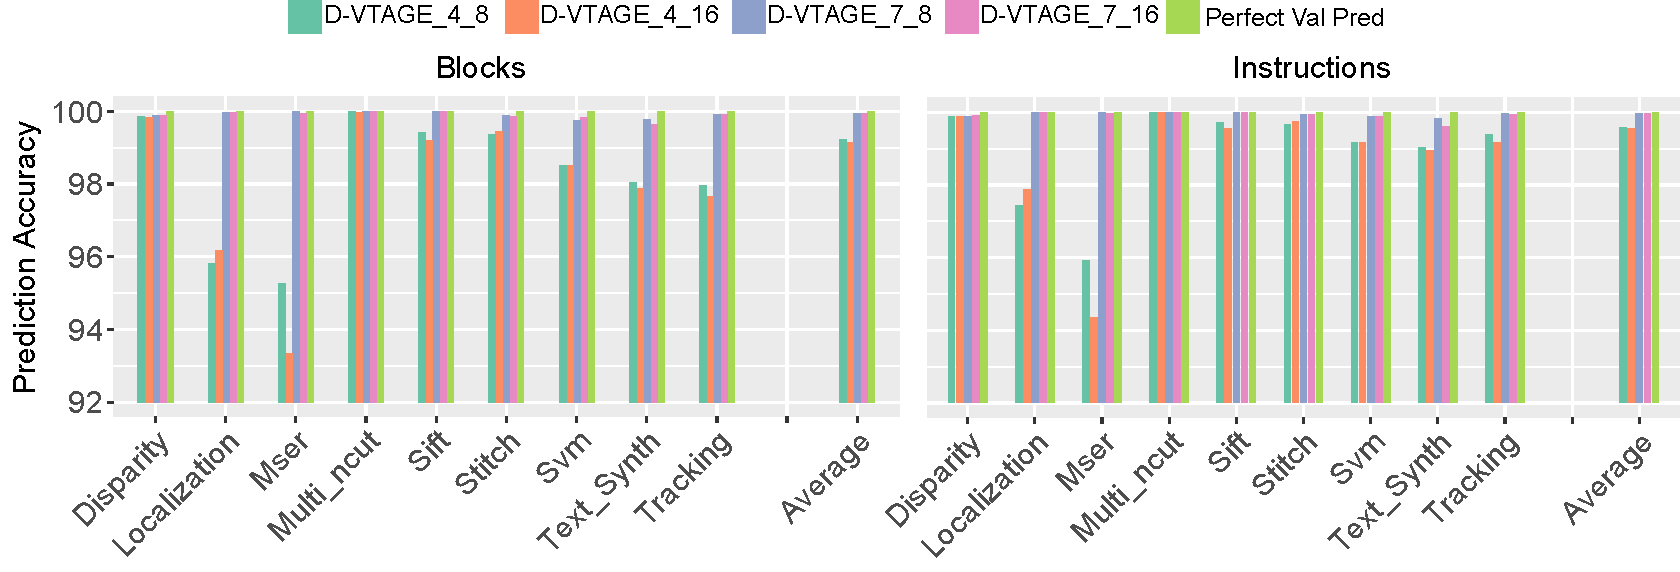
\includegraphics[width=1\textwidth]{chapter3/graphics/predAcc.pdf}
    \caption{Accuracy of the different D-VTAGE predictors at a block and instruction level. Higher is better.}
    \label{fig:vtag_accuracy_block}
	\vspace{1em}
\end{figure}

The coverage shows that a lower confidence allows for higher coverage, yet the speedups seen in Figure~\ref{fig:vtage_perf} indicate that a higher confidence leads to better performance.
Intuitively, this must mean that the lower confidence leads to higher misprediction.
To confirm this, Figures~\ref{fig:vtag_accuracy_block} shows the misprediction rate (in percentage) for each benchmark at a per-block and per-instruction base respectively.

The accuracy Figures show that overall, the D-VTAGE predictor maintains a 99\% accuracy, whether at the block level or instruction level.
However, for \bm{Localization}, \bm{MSER}, \bm{SVM}, \bm{Texture\_Synthesis} and \bm{Tracking}, the block level accuracy for a confidence of 4 is under 98\%, and even down to 93\% for \bm{MSER}.
The effect of a value misprediction is similar to a branch misprediction: it causes a flush of all blocks younger than the block with the incorrect misprediction.
Therefore, just like branch prediction, large core compositions are very sensitive to mispredictions.
This explains why the low confidence counter sometimes performs worse than the higher confidence as it mispredicts more often.

\subsubsection{Size of stride}

\begin{figure}[t]
    \centering
    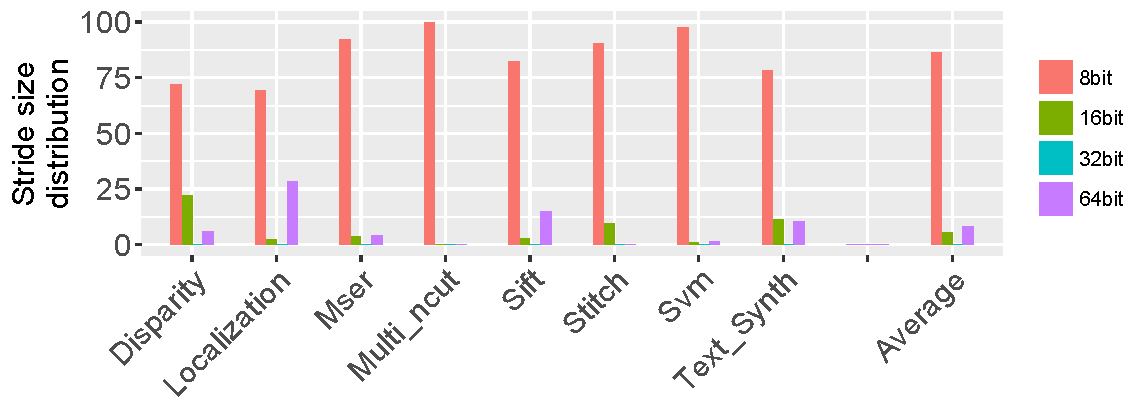
\includegraphics[width=1\textwidth]{chapter3/graphics/strides.pdf}
    \caption{Distribution of the size of strides for each benchmark.}
    \label{fig:strides}
	\vspace{1em}
\end{figure}

Finally, whilst 64 bit strides are used throughout the experiments to capture all the potential performance, 64 bits per entries may not be necessary.
Figure~\ref{fig:strides} shows the average number of valid predictions whose strides could fit in either an 8, 16, 32 or 64 bit signed integer for each of the benchmarks.
The data was taken from the D-VTAGE configuration that led to the highest performance overall for each of the benchmarks.
In Perais' et al'.s work they recommend that a medium-sized D-VTAGE predictor use 8-bit strides.
Overall, Figure~\ref{fig:strides} shows that using 8 bit strides should be sufficient for most benchmarks, however \bm{Disparity}, one of the benchmarks which benefits most from value prediction, would lose almost 25\% of its coverage.
Therefore, for these set of applications, a stride of at least 16 bits is necessary.

\subsection{Summary}
